%% LyX 2.4.4 created this file.  For more info, see https://www.lyx.org/.
%% Do not edit unless you really know what you are doing.
\documentclass[english,t]{beamer}
\usepackage{mathptmx}
\usepackage[T1]{fontenc}
\usepackage[latin9]{inputenc}
\usepackage{amssymb}
\usepackage{cancel}
\usepackage{graphicx}

\makeatletter

%%%%%%%%%%%%%%%%%%%%%%%%%%%%%% LyX specific LaTeX commands.
%% Because html converters don't know tabularnewline
\providecommand{\tabularnewline}{\\}

%%%%%%%%%%%%%%%%%%%%%%%%%%%%%% Textclass specific LaTeX commands.
% this default might be overridden by plain title style
\newcommand\makebeamertitle{\frame{\maketitle}}%
% (ERT) argument for the TOC
\AtBeginDocument{%
  \let\origtableofcontents=\tableofcontents
  \def\tableofcontents{\@ifnextchar[{\origtableofcontents}{\gobbletableofcontents}}
  \def\gobbletableofcontents#1{\origtableofcontents}
}

%%%%%%%%%%%%%%%%%%%%%%%%%%%%%% User specified LaTeX commands.
\usetheme{Warsaw}
% or ...

\setbeamercovered{transparent}
% or whatever (possibly just delete it)
\setbeamercovered{invisible} %makes overlays invisible


%gets rid of navigation symbols
\setbeamertemplate{navigation symbols}{}

\usepackage{multicol}

\usepackage{tikz}
\usetikzlibrary{plotmarks}
\usepackage{pgfplots}
\pgfplotsset{compat=newest}

\usepackage{calc}
\usepackage[nomessages]{fp}

\usepackage{advdate}    % Advancing/saving dates
\usepackage{datetime}   % Dates formatting
\usepackage{datenumber} % Counters for dates

%\usepackage{pgfpages}
%\pgfpagesuselayout{4 on 1}[a4paper, landscape, border shrink=7mm]
%\pgfpageslogicalpageoptions{1}{border code=\pgfusepath{stroke}}
%\pgfpageslogicalpageoptions{2}{border code=\pgfusepath{stroke}}
%\pgfpageslogicalpageoptions{3}{border code=\pgfusepath{stroke}}
%\pgfpageslogicalpageoptions{4}{border code=\pgfusepath{stroke}}
%%%Don't forget to add 'handout'

\makeatother

\usepackage{babel}
\begin{document}
\newcommand{\chNum}{1}
\newcommand{\secNum}{1}

\newcommand{\xmax}{6}
\newcommand{\xmin}{-6}
\newcommand{\xstep}{0} %must be xmin+n
\newcommand{\ymax}{6}
\newcommand{\ymin}{-6}
\newcommand{\ystep}{0} %must be ymin+n

\newcounter{countEx} \setcounter{countEx}{0}
\newcounter{countProb} \setcounter{countProb}{0}
\resetcounteronoverlays{countEx} \resetcounteronoverlays{countProb}

\newcommand{\ex}[3]{
	\addtocounter{countEx}{1}
	\only<#1-#2>{\begin{exampleblock} {Example \chNum.\secNum.\arabic{countEx}.} #3	\end{exampleblock}}
}

\newcommand{\prob}[4]{
	\addtocounter{countProb}{1}
	\only<#1-#2>{\begin{exampleblock} {Ex.\, \chNum.\secNum.\arabic{countProb}.\,#3} #4	\end{exampleblock}}
}
\title[Section 1.1: Slopes and Equations of Lines]{Section 1.1: Slopes and Equations of Lines }
\subtitle{Finite Mathematics~~MTH 132~~Spring 2014}
\author{Dr.\,James Ashe}
\titlegraphic{\includegraphics[height=1.5cm]{D:/home/jim/JamesAshe/JCSU/images/jcsu_bull.jpg}}
\institute{Johnson C. Smith University}
\date{{}}

\makebeamertitle

\beamerdefaultoverlayspecification{<+->}
\begin{frame}{Chapter 1 Outline}

\textbf{Chapter 1: Linear Functions}
\begin{itemize}
\item []<2->1.1 Slopes and Equations of Lines
\item []<3->1.2 Linear Functions \& Applications
\item []<4->1.3 Least Squares Line
\end{itemize}
\end{frame}

\begin{frame}{Linear Equations/Functions}

\begin{columns}


\column{5.75cm}

What is a linear functions?
\begin{itemize}
\item <2->Equations are functions.

\begin{itemize}
\item [ex.]<3->$y=2x-3$
\item []<4->$f(x)=2x-3$
\end{itemize}
\item <5->The graph of a linear function is \emph{always a line.}
\item <6->The \emph{rate of change }is constant.

\begin{itemize}
\item [ex.]<7->%
\begin{tabular}{l|rl}
$x$ & $f(x)$ & \tabularnewline
\cline{1-2}
$0$ & $-3$ & $f(0)=2(0)-3=-3$\tabularnewline
$1$ & $-1$ & $f(1)=2(1)-3=-1$\tabularnewline
$2$ & $1$ & $f(2)=2(2)-3=1$\tabularnewline
\end{tabular}
\end{itemize}
\end{itemize}

\column{6cm}

\vspace{-.5cm}
%%%%%%%
\begin{tikzpicture} 
\begin{axis}[height=5.5cm, 
	width=5.5cm, axis lines=middle,
	minor x tick num={4},
	minor y tick num={4},
	grid=both,
	%xtick={0,50,...,250},
	%ytick={0,10,20,...,40},
	%axis line style={-latex}, 
	xmin=\xmin,xmax=\xmax, 
	ymin=\ymin,ymax=\ymax,
	%restrict y to domain=-1:10,
	%no markers, 
	xlabel={$x$},ylabel={$y$}, 
	%every axis x label/.append style={anchor=north}, 
	%every axis y label/.append style={anchor=east}
	]
  
	\only<3->{\addplot[domain=\xmin:\xmax,thick,draw=red,<->]{2*x-3} node[pos=.65,above] {$$};}
	\only<8->{\addplot[color=blue,solid,mark=*,style={font=\footnotesize}] coordinates {(0,-3)} node[left] {$(0,-3)$};}
	\only<9->{\addplot[color=blue,solid,mark=*,style={font=\footnotesize}] coordinates {(1,-1)} node[right] {$(1,-1)$};}
	\only<10->{\addplot[color=blue,solid,mark=*,style={font=\footnotesize}] coordinates {(2,1)} node[above,right] {$(2,1)$};}
	
\end{axis}
\end{tikzpicture}
\end{columns}
\end{frame}

\begin{frame}{Slope of a Line}

\begin{columns}


\column{5.5cm}
\begin{block}{Slope of a Line}
The \emph{slope of a line }is the ratio of the vertical change to
horizontal change. $m=\frac{y_{2}-y_{1}}{x_{2}-x_{1}}$
\end{block}
\ex{1}{1}{$(1,-1)$ and $(2,1)$}
\ex{2}{2}{$(1,3)$ and $(2,3)$}
\ex{3}{3}{$(2,4)$ and $(2,1)$}

\column{5.5cm}

\end{columns}
\end{frame}

\begin{frame}{Find the equation of a Line}

\begin{columns}


\column{5.5cm}
\begin{block}{Slope-intecept Form}

\centering$y=mx+b$
\end{block}
\vspace{0cm}
\begin{block}<2->{Point-Slope Formula}
 \centering$y-y_{1}=m(x-x_{1})$
\end{block}
\begin{itemize}
\item <3->$m$ is the slope.
\item <4->$b$ is the $y$-int.
\end{itemize}
\ex{5}{5}{Find the slope-int.\, form of the line with a slope of $-3$ passing through $(6,6)$.}
\ex{6}{6}{find the equation of the line which passes through $(-2,5)$ and $(3,6)$.}
\ex{7}{7}{Find the equation of the line that is \emph{parallel} to $y=x+1$ and passes through $(0,2)$.}
\ex{8}{8}{Find the equation of the line that is \emph{perpendicular} to $y= \frac{2}{3}+1$ and passes through $(0,2)$.}

\column{5.5cm}

\end{columns}
\end{frame}

\begin{frame}{}

\begin{block}{Summary}
\begin{tabular}{rl}
\textbf{Equation} & \textbf{Description}\tabularnewline
$y=mx+b$ & \textbf{Slope-int.\,form }slope $m$, $y$-int $b$\tabularnewline
$y-y_{1}=m(x-x_{1})$ & \textbf{Pt-slope formula }passing through $(x_{1},y_{1})$\tabularnewline
$y=k$ & \textbf{Horizontal line }through $(x,k)$\tabularnewline
$x=k$ & \textbf{Vertical line }through $(k,y)$\tabularnewline
$m=\frac{a}{b}$ & if \textbf{parallel }to $y=\frac{a}{b}x+b$\tabularnewline
$m=-\frac{b}{a}$ & if \textbf{perpendicular }to $y=\frac{a}{b}x+b$\tabularnewline
\end{tabular}
\end{block}
\prob{2}{}{Use the conditions to write an equation for the line in slope-int.\, form.}{Slope$=-3$, $m$ passing through $(6,6)$.}

\prob{2}{}{Use the conditions to write an equation for the line in slope-int.\, form.}{Perpendicular to $y=-\frac{1}{2}x+7$ passing through $(7,3)$.}
\end{frame}

\begin{frame}{Modeling with Linear Functions }

\begin{columns}


\column{5.5cm}

\begin{tabular}{|c|c|}
\hline 
\textbf{Year} & \textbf{Cost of College}\tabularnewline
\hline 
2000 & 3508\tabularnewline
\hline 
2002 & 4098\tabularnewline
\hline 
2004 & 5126\tabularnewline
\hline 
2006 & 5804\tabularnewline
\hline 
2008 & 6591\tabularnewline
\hline 
\end{tabular}

\column{5.5cm}

\vspace{-.5cm}
%%%%%%%
\begin{tikzpicture} 
\begin{axis}[height=5.5cm, 
	width=5.5cm, axis lines=middle,
	minor x tick num={4},minor y tick num={4},
	grid=both,
	%xmin=\xmin,xmax=\xmax,ymin=\ymin,ymax=\ymax,
	xlabel={$year$},ylabel={$cost$}, 
	%xtick={0,50,...,250},%ytick={0,10,20,...,40},%axis line style={-latex}, 
	%restrict y to domain=-1:10,%no markers, 
	%every axis x label/.append style={anchor=north},%every axis y label/.append style={anchor=east}
	]
  
	%\only<2->{\addplot[thick,draw=red,<->]{2*x-3} node[pos=.65,above] {$$};}
	\only<2->{\addplot[color=blue,solid,mark=*,style={font=\footnotesize}] coordinates {(2000,3508)};}
	\only<3->{\addplot[color=blue,solid,mark=*,style={font=\footnotesize}] coordinates {(2000,3508) (2002,4098) (2004,5126) (2006,5804) (2008,6591)};}
	\only<4->{\addplot[color=red,thick,solid,mark=*,style={font=\footnotesize}] coordinates {(2000,3508) (2008,6591)};}
	
\end{axis}
\end{tikzpicture}
\end{columns}
\end{frame}

\end{document}
